\documentclass{standalone}
\usepackage{tikz}
\usetikzlibrary{patterns, positioning}


\begin{document}
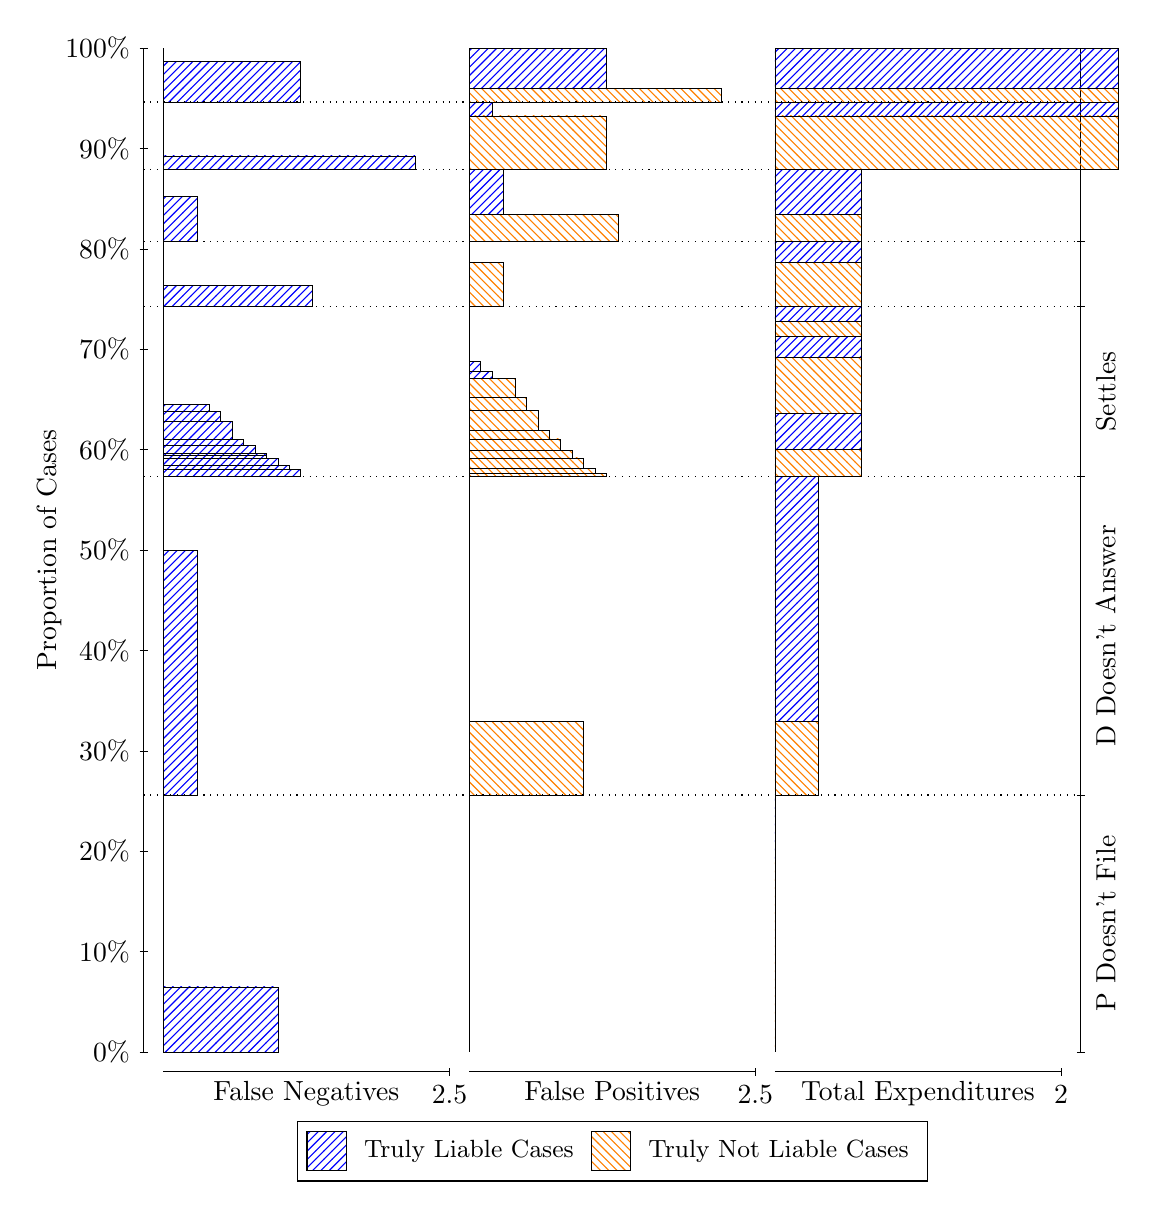
\begin{tikzpicture}
\draw[black, very thin] (1.5,1.75) -- (1.5,14.5);
\node[rotate=90, text=black, anchor=center] at (0.3, 8.125) {Proportion of Cases};
\draw[black, very thin] (1.45,1.75) -- (1.55,1.75);
\node[text=black, anchor=east] at (1.45, 1.75) {0\%};
\draw[black, very thin] (1.45,3.025) -- (1.55,3.025);
\node[text=black, anchor=east] at (1.45, 3.025) {10\%};
\draw[black, very thin] (1.45,4.3) -- (1.55,4.3);
\node[text=black, anchor=east] at (1.45, 4.3) {20\%};
\draw[black, very thin] (1.45,5.575) -- (1.55,5.575);
\node[text=black, anchor=east] at (1.45, 5.575) {30\%};
\draw[black, very thin] (1.45,6.85) -- (1.55,6.85);
\node[text=black, anchor=east] at (1.45, 6.85) {40\%};
\draw[black, very thin] (1.45,8.125) -- (1.55,8.125);
\node[text=black, anchor=east] at (1.45, 8.125) {50\%};
\draw[black, very thin] (1.45,9.4) -- (1.55,9.4);
\node[text=black, anchor=east] at (1.45, 9.4) {60\%};
\draw[black, very thin] (1.45,10.675) -- (1.55,10.675);
\node[text=black, anchor=east] at (1.45, 10.675) {70\%};
\draw[black, very thin] (1.45,11.95) -- (1.55,11.95);
\node[text=black, anchor=east] at (1.45, 11.95) {80\%};
\draw[black, very thin] (1.45,13.225) -- (1.55,13.225);
\node[text=black, anchor=east] at (1.45, 13.225) {90\%};
\draw[black, very thin] (1.45,14.5) -- (1.55,14.5);
\node[text=black, anchor=east] at (1.45, 14.5) {100\%};

\draw[black, very thin] (13.4,1.75) -- (13.4,14.5);
\draw[black, very thin] (13.35,1.75) -- (13.45,1.75);
\node[anchor=west] at (13.35, 1.75) {};
\draw[black, very thin] (13.35,5.014) -- (13.45,5.014);
\node[anchor=west] at (13.35, 5.014) {};
\draw[black, very thin] (13.35,9.0574) -- (13.45,9.0574);
\node[anchor=west] at (13.35, 9.0574) {};
\draw[black, very thin] (13.35,11.219) -- (13.45,11.219);
\node[anchor=west] at (13.35, 11.219) {};
\draw[black, very thin] (13.35,12.046) -- (13.45,12.046);
\node[anchor=west] at (13.35, 12.046) {};
\draw[black, very thin] (13.35,12.955) -- (13.45,12.955);
\node[anchor=west] at (13.35, 12.955) {};
\draw[black, very thin] (13.35,13.814) -- (13.45,13.814);
\node[anchor=west] at (13.35, 13.814) {};
\draw[black, very thin] (13.35,14.5) -- (13.45,14.5);
\node[anchor=west] at (13.35, 14.5) {};

\draw[black, very thin, pattern color=blue, pattern=north east lines] (1.75,1.75) rectangle (3.2033,2.5765);
\draw[black, very thin, pattern color=orange, pattern=north west lines] (1.75,2.5765) rectangle (1.75,5.014);
\draw[black, very thin, pattern color=blue, pattern=north east lines] (1.75,5.014) rectangle (2.186,8.125);
\draw[black, very thin, pattern color=orange, pattern=north west lines] (1.75,8.125) rectangle (1.75,9.0574);
\draw[black, very thin, pattern color=blue, pattern=north east lines] (1.75,9.0574) rectangle (3.494,9.1447);
\draw[black, very thin, pattern color=blue, pattern=north east lines] (1.75,9.1447) rectangle (3.3487,9.2032);
\draw[black, very thin, pattern color=blue, pattern=north east lines] (1.75,9.2032) rectangle (3.2033,9.2866);
\draw[black, very thin, pattern color=blue, pattern=north east lines] (1.75,9.2866) rectangle (3.058,9.328);
\draw[black, very thin, pattern color=blue, pattern=north east lines] (1.75,9.328) rectangle (3.058,9.3539);
\draw[black, very thin, pattern color=blue, pattern=north east lines] (1.75,9.3539) rectangle (2.9127,9.4543);
\draw[black, very thin, pattern color=blue, pattern=north east lines] (1.75,9.4543) rectangle (2.7673,9.5299);
\draw[black, very thin, pattern color=blue, pattern=north east lines] (1.75,9.5299) rectangle (2.622,9.761);
\draw[black, very thin, pattern color=blue, pattern=north east lines] (1.75,9.761) rectangle (2.4767,9.8857);
\draw[black, very thin, pattern color=blue, pattern=north east lines] (1.75,9.8857) rectangle (2.3313,9.9763);
\draw[black, very thin, pattern color=orange, pattern=north west lines] (1.75,9.9763) rectangle (1.75,11.219);
\draw[black, very thin, pattern color=blue, pattern=north east lines] (1.75,11.219) rectangle (3.6393,11.485);
\draw[black, very thin, pattern color=orange, pattern=north west lines] (1.75,11.485) rectangle (1.75,12.046);
\draw[black, very thin, pattern color=blue, pattern=north east lines] (1.75,12.046) rectangle (2.186,12.612);
\draw[black, very thin, pattern color=orange, pattern=north west lines] (1.75,12.612) rectangle (1.75,12.955);
\draw[black, very thin, pattern color=blue, pattern=north east lines] (1.75,12.955) rectangle (4.9473,13.129);
\draw[black, very thin, pattern color=orange, pattern=north west lines] (1.75,13.129) rectangle (1.75,13.814);
\draw[black, very thin, pattern color=blue, pattern=north east lines] (1.75,13.814) rectangle (3.494,14.326);
\draw[black, very thin, pattern color=orange, pattern=north west lines] (1.75,14.326) rectangle (1.75,14.5);
\draw[black, very thin, pattern color=orange, pattern=north west lines] (5.6333,1.75) rectangle (5.6333,4.1875);
\draw[black, very thin, pattern color=blue, pattern=north east lines] (5.6333,4.1875) rectangle (5.6333,5.014);
\draw[black, very thin, pattern color=orange, pattern=north west lines] (5.6333,5.014) rectangle (7.0867,5.9464);
\draw[black, very thin, pattern color=blue, pattern=north east lines] (5.6333,5.9464) rectangle (5.6333,9.0574);
\draw[black, very thin, pattern color=orange, pattern=north west lines] (5.6333,9.0574) rectangle (7.3773,9.0961);
\draw[black, very thin, pattern color=orange, pattern=north west lines] (5.6333,9.0961) rectangle (7.232,9.161);
\draw[black, very thin, pattern color=orange, pattern=north west lines] (5.6333,9.161) rectangle (7.0867,9.2936);
\draw[black, very thin, pattern color=orange, pattern=north west lines] (5.6333,9.2936) rectangle (6.9413,9.3904);
\draw[black, very thin, pattern color=orange, pattern=north west lines] (5.6333,9.3904) rectangle (6.796,9.5368);
\draw[black, very thin, pattern color=orange, pattern=north west lines] (5.6333,9.5368) rectangle (6.6507,9.6466);
\draw[black, very thin, pattern color=orange, pattern=north west lines] (5.6333,9.6466) rectangle (6.5053,9.9005);
\draw[black, very thin, pattern color=orange, pattern=north west lines] (5.6333,9.9005) rectangle (6.36,10.065);
\draw[black, very thin, pattern color=orange, pattern=north west lines] (5.6333,10.065) rectangle (6.2147,10.3);
\draw[black, very thin, pattern color=blue, pattern=north east lines] (5.6333,10.3) rectangle (5.924,10.391);
\draw[black, very thin, pattern color=blue, pattern=north east lines] (5.6333,10.391) rectangle (5.7787,10.516);
\draw[black, very thin, pattern color=blue, pattern=north east lines] (5.6333,10.516) rectangle (5.6333,11.219);
\draw[black, very thin, pattern color=orange, pattern=north west lines] (5.6333,11.219) rectangle (6.0693,11.78);
\draw[black, very thin, pattern color=blue, pattern=north east lines] (5.6333,11.78) rectangle (5.6333,12.046);
\draw[black, very thin, pattern color=orange, pattern=north west lines] (5.6333,12.046) rectangle (7.5227,12.389);
\draw[black, very thin, pattern color=blue, pattern=north east lines] (5.6333,12.389) rectangle (6.0693,12.955);
\draw[black, very thin, pattern color=orange, pattern=north west lines] (5.6333,12.955) rectangle (7.3773,13.639);
\draw[black, very thin, pattern color=blue, pattern=north east lines] (5.6333,13.639) rectangle (5.924,13.814);
\draw[black, very thin, pattern color=orange, pattern=north west lines] (5.6333,13.814) rectangle (8.8307,13.988);
\draw[black, very thin, pattern color=blue, pattern=north east lines] (5.6333,13.988) rectangle (7.3773,14.5);
\draw[black, very thin, pattern color=orange, pattern=north west lines] (9.5167,1.75) rectangle (9.5167,4.1875);
\draw[black, very thin, pattern color=blue, pattern=north east lines] (9.5167,4.1875) rectangle (9.5167,5.014);
\draw[black, very thin, pattern color=orange, pattern=north west lines] (9.5167,5.014) rectangle (10.062,5.9464);
\draw[black, very thin, pattern color=blue, pattern=north east lines] (9.5167,5.9464) rectangle (10.062,9.0574);
\draw[black, very thin, pattern color=orange, pattern=north west lines] (9.5167,9.0574) rectangle (10.607,9.4013);
\draw[black, very thin, pattern color=blue, pattern=north east lines] (9.5167,9.4013) rectangle (10.607,9.8576);
\draw[black, very thin, pattern color=orange, pattern=north west lines] (9.5167,9.8576) rectangle (10.607,10.569);
\draw[black, very thin, pattern color=blue, pattern=north east lines] (9.5167,10.569) rectangle (10.607,10.839);
\draw[black, very thin, pattern color=orange, pattern=north west lines] (9.5167,10.839) rectangle (10.607,11.027);
\draw[black, very thin, pattern color=blue, pattern=north east lines] (9.5167,11.027) rectangle (10.607,11.219);
\draw[black, very thin, pattern color=orange, pattern=north west lines] (9.5167,11.219) rectangle (10.607,11.78);
\draw[black, very thin, pattern color=blue, pattern=north east lines] (9.5167,11.78) rectangle (10.607,12.046);
\draw[black, very thin, pattern color=orange, pattern=north west lines] (9.5167,12.046) rectangle (10.607,12.389);
\draw[black, very thin, pattern color=blue, pattern=north east lines] (9.5167,12.389) rectangle (10.607,12.955);
\draw[black, very thin, pattern color=orange, pattern=north west lines] (9.5167,12.955) rectangle (13.877,13.639);
\draw[black, very thin, pattern color=blue, pattern=north east lines] (9.5167,13.639) rectangle (13.877,13.814);
\draw[black, very thin, pattern color=orange, pattern=north west lines] (9.5167,13.814) rectangle (13.877,13.988);
\draw[black, very thin, pattern color=blue, pattern=north east lines] (9.5167,13.988) rectangle (13.877,14.5);
\draw[black, dotted] (1.5,5.014) -- (13.4,5.014);
\draw[black, dotted] (1.5,9.0574) -- (13.4,9.0574);
\draw[black, dotted] (1.5,11.219) -- (13.4,11.219);
\draw[black, dotted] (1.5,12.046) -- (13.4,12.046);
\draw[black, dotted] (1.5,12.955) -- (13.4,12.955);
\draw[black, dotted] (1.5,13.814) -- (13.4,13.814);
\draw[black, very thin] (1.75,1.5) -- (5.3833,1.5);
\node[text=black, anchor=north] at (3.5667, 1.5) {False Negatives};
\draw[black, very thin] (5.3833,1.45) -- (5.3833,1.55);
\node[text=black, anchor=north] at (5.3833, 1.45) {2.5};

\draw[black, very thin] (5.6333,1.5) -- (9.2667,1.5);
\node[text=black, anchor=north] at (7.45, 1.5) {False Positives};
\draw[black, very thin] (9.2667,1.45) -- (9.2667,1.55);
\node[text=black, anchor=north] at (9.2667, 1.45) {2.5};

\draw[black, very thin] (9.5167,1.5) -- (13.15,1.5);
\node[text=black, anchor=north] at (11.333, 1.5) {Total Expenditures};
\draw[black, very thin] (13.15,1.45) -- (13.15,1.55);
\node[text=black, anchor=north] at (13.15, 1.45) {2};

\node[text=black, centered, rotate=90] at (13.72, 3.382) {P Doesn't File};
\node[text=black, centered, rotate=90] at (13.72, 7.0357) {D Doesn't Answer};
\node[text=black, centered, rotate=90] at (13.72, 10.138) {Settles};





\draw (7.449999999999999,1.5) node[draw=none] (baseCoordinate) {};
\begin{scope}[align=center]
        \matrix[scale=0.5, draw=black, below=0.5cm of baseCoordinate, nodes={draw}, column sep=0.1cm]{
            \node[rectangle, draw, minimum width=0.5cm, minimum height=0.5cm, pattern color=blue, pattern=north east lines] {}; &
            \node[draw=none, font=\small, text=black] (B) {Truly Liable Cases}; &
            \node[rectangle, draw, minimum width=0.5cm, minimum height=0.5cm, pattern color=orange, pattern=north west lines] {}; &
            \node[draw=none, font=\small, text=black] (B) {Truly Not Liable Cases}; \\
            };
\end{scope}

\end{tikzpicture}
\end{document}